%; whizzy chapter -dvi
% -initex iniptex -latex platex -format platex -bibtex jbibtex -fmt fmt
% 以上 whizzytex を使用する場合の設定。
 
%     Tokyo Debian Meeting resources
%     Copyright (C) 2012 Junichi Uekawa
%     Copyright (C) 2011 Nobuhiro Iwamatsu

%     This program is free software; you can redistribute it and/or modify
%     it under the terms of the GNU General Public License as published by
%     the Free Software Foundation; either version 2 of the License, or
%     (at your option) any later version.

%     This program is distributed in the hope that it will be useful,
%     but WITHOUT ANY WARRANTY; without even the implied warranty of
%     MERCHANTABILITY or FITNESS FOR A PARTICULAR PURPOSE.  See the
%     GNU General Public License for more details.

%     You should have received a copy of the GNU General Public License
%     along with this program; if not, write to the Free Software
%     Foundation, Inc., 51 Franklin St, Fifth Floor, Boston, MA  02110-1301 USA

%  preview (shell-command (concat "evince " (replace-regexp-in-string "tex$" "pdf"(buffer-file-name)) "&"))

%%ここからヘッダ開始。

\documentclass[mingoth,a4paper]{jsarticle}
\usepackage{monthlyreport}
% 日付を定義する、毎月変わります。
\newcommand{\debmtgyear}{2014}
\newcommand{\debmtgmonth}{04}
\newcommand{\debmtgdate}{19}
% started from zero:
% (let ((year 2013) (month 7)) (+ (* (- year 2005) 12) month -1))
\newcommand{\debmtgnumber}{112}

\begin{document}

\begin{titlepage}
\thispagestyle{empty}
% タイトルページ:編集必要な部分は最初のマクロに飛ばすこと

\vspace*{-2cm}
第\debmtgnumber{}回 東京エリア Debian 勉強会資料\\
\hspace*{-2cm}
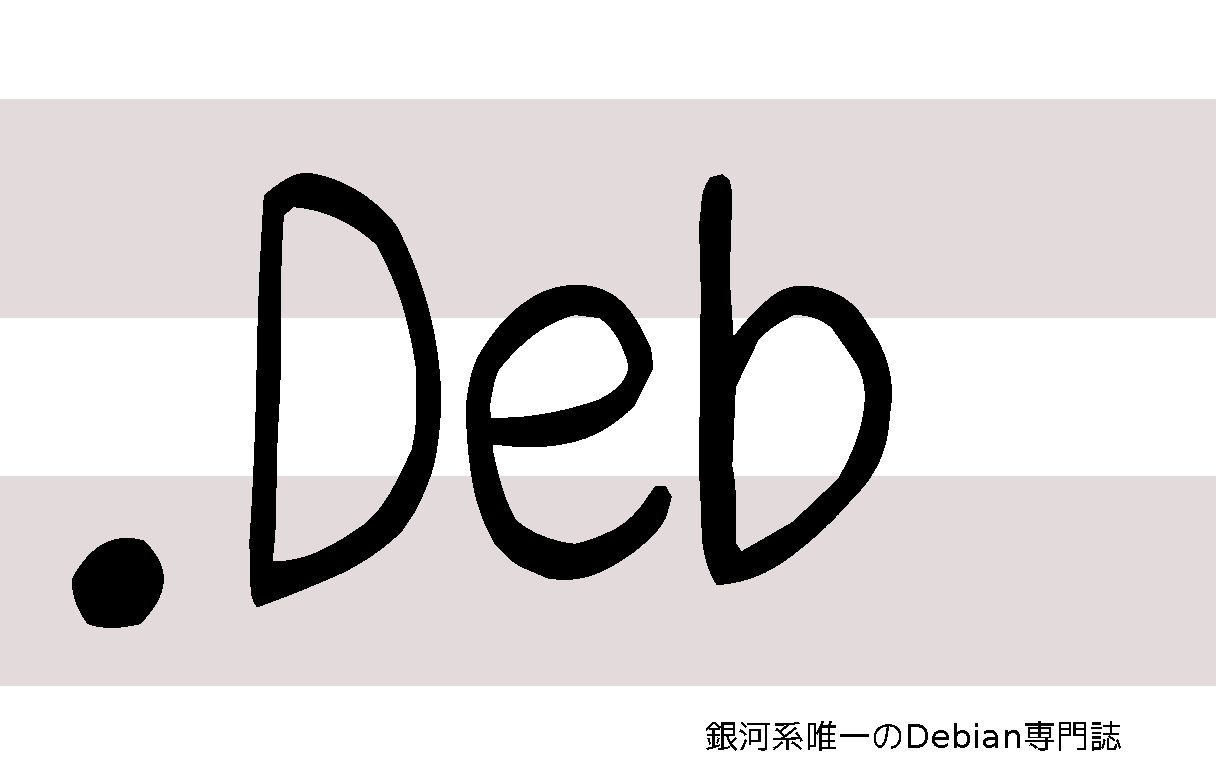
\includegraphics{image2012-natsu/dotdeb.pdf}\\
\hfill{}\debmtgyear{}年\debmtgmonth{}月\debmtgdate{}日

% ここはアップデートすること
% 全角文字にしないとフォントのサイズが合わないので注意
\rotatebox{10}{\fontsize{32}{32} {\gt 特集:Golangなツールのパッケージ化}}\\
\rotatebox{10}{\fontsize{32}{32} {\gt (Serf編)}}\\

\vspace*{-2cm}
\hfill{}
\includegraphics[height=6cm]{image200502/openlogo-nd.eps}
\end{titlepage}

\newpage

\begin{minipage}[b]{0.2\hsize}
 \definecolor{titleback}{gray}{0.9}
 \colorbox{titleback}{\rotatebox{90}{\fontsize{80}{80} {\gt デビアン勉強会} }}
\end{minipage}
\begin{minipage}[b]{0.8\hsize}
\hrule
\vspace{2mm}
\hrule
\begin{multicols}{2}
\tableofcontents
\end{multicols}
\vspace{2mm}
\hrule
\end{minipage}

\dancersection{事前課題}{野島 貴英}

今回の事前課題は以下です:
\begin{enumerate}
 \item 本日、何の作業をやるかを宣言ください。
\end{enumerate}
この課題に対して提出いただいた内容は以下です。
\begin{multicols}{2}
{\small
\begin{prework}{ 野島貴英 }

\begin{itemize}
\item Xmrisパッケージ化頑張る
\item iOS7.1 debian接続再び。
\end{itemize}
\end{prework}

\begin{prework}{ 岩松 信洋 }

?

\end{prework}

\begin{prework}{ dictoss(杉本 典充) }

Debian上でLeap Motionを動かしてみる

\end{prework}

\begin{prework}{ Yoshida Shin }

GitHub に公開しているプログラムの機能追加。
動作環境は Debian Sid で。
\end{prework}

\begin{prework}{ Koji Hasebe }

Debianパッケージ作成の方法を調査し、実際に作成する。
アウトプットとして、その方法を手順書にまとめる。
\end{prework}

\begin{prework}{ henrich }
\begin{itemize}
\item OSC北海道用の資料作成
\item debhelperの査読の続き
\item パッケージまわりでのなにか
\end{itemize}
のいずれか。

\end{prework}

\begin{prework}{ zinrai }

Debianパッケージ作成。
\begin{itemize}
\item Debianパッケージ作成してみたい
\item 「Debianパッケージング道場」に都合がつかず参加できなかったので「もくもく会」の時間を使いパッケージ作成の作法を心得ている人がいる環境でパッケージ作成したい
\item redis 2.8.8をDebianパッケージ作成の題材にしてみようと思う。
\url{http://redis.io/}
\item 通勤時間などを使い当日までにこの辺に目を通しておきたい
\url{http://www.debian.or.jp/community/devel/}
\end{itemize}
\end{prework}

\begin{prework}{ yyuu }

自分で管理してるプロジェクトのdeb化を要望されてしまったので、そのための作業を行ないたいと考えています。

\url{https://github.com/yyuu/pyenv/issues/138}

\end{prework}

\begin{prework}{ 野首(@knok) }
\begin{itemize}
\item KAKASIローマ字テーブルの改善
\item LanguageToolのルール追加
\item gnu.org, veの翻訳
\end{itemize}
\end{prework}

\begin{prework}{ まえだこうへい }

\begin{itemize}
\item Golang関係のパッケージ化の話をする
\item \url{http://qa.debian.org/developer.php?login=mkouhei@palmtb.net}
のバグ潰し&パッケージアップデート
\item 上記のGolang関係のパッケージをpkg-go teamでのメンテナンスを始める(MLに投稿&ITPする)
\end{itemize}
\end{prework}

}
\end{multicols}

\dancersection{Debian Trivia Quiz}{野島 貴英}

ところで、みなさん Debian 関連の話題においついていますか?Debian関連の話
題はメーリングリストをよんでいると追跡できます。ただよんでいるだけではは
りあいがないので、理解度のテストをします。特に一人だけでは意味がわからな
いところもあるかも知れません。みんなで一緒に読んでみましょう。

今回の出題範囲は\url{debian-devel-announce@lists.debian.org} や \url{debian-devel@lists.debian.org}に投稿された
内容などからです。

\begin{multicols}{2}
%; whizzy-master ../debianmeetingresume201311.tex
% $B0J>e$N@_Dj$r$7$F$$$k$?$a!"$3$N%U%!%$%k$G(B M-x whizzytex $B$9$k$H!"(Bwhizzytex$B$,MxMQ$G$-$^$9!#(B
%

\santaku
{2015$BG/$N(BDebconf15$B$N3+:E9q$O$I$3$K$J$C$?$G$7$g$&!)(B}
{$B%\%9%K%"!&%X%k%D%'%4%S%J(B}
{$B%&%/%i%$%J(B}
{$B%I%$%D(B}
{C}
{$B:#EY$O%I%$%D$@$=$&$G$9!#$A$J$_$K:#G/$N(BDebconf14$B$O(B8/23-31$B$G(BUSA$B$N(BPortland,Oregon
$B$G3+:EM=Dj$G$9!#(B}

\santaku
{DPL$BA*5s$,9T$o$l$^$7$?!#:#G/$N(BDPL$B$OC/$K$J$C$?$G$7$g$&$+!)(B}
{Lucas Nussbaum}
{Neil McGovern}
{Rapha\"{e}l Hertzog}
{A}
{$B:#G/$N(BDPL$B$N8uJd<T$O#2L>$G!"(BLucas Nussbaum$B$5$s!"(BNeil McGovern$B$5$s$N#2L>(B
$B$G$7$?!##2L>$H$b<+A&$H$N$3$H$G$9!#A*5s$N7k2L!"(B
Lucas Nussbaum(lucus)$B$5$s$N05>!$@$C$?$h$&$G$9!#$A$J$_$K!"(B
Rapha\"{e}l Hertzog$B$5$s$O!"(BThe Debian 
Administrator\'s handbook$B$N:n<T!"B>$K$b0N6H$,$?$/$5$s!#(B}

\santaku
{clang3.4$B$K$h$k(BDebian$B%Q%C%1!<%8$N:F9=C[$,9T$o$l$^$7$?!#7k2L2?(B\%$B$N%Q%C%1!<%8$,@.8y$7$?$G$7$g$&$+!)(B}
{90\%}
{50\%}
{10\%}
{A}
{\url{http://clang.debian.net/}$B$,(Bclang$B$K$h$k(BDebian$B%Q%C%1!<%8:F9=C[$N%]!<%?%k%5%$%H$G$9!#KhG/!"(Bclang$B$N%P!<%8%g%s$r>e$2$F!"A4(BDebian$B%Q%C%1!<%8$r:F9=C[$7$?7k2L$,:\$j$^$9!#:#G/$N7k2L$H$7$F$O:F9=C[BP>]$N%Q%C%1!<%8$N?t$,5nG/$HBgI}$KA}$($F$$$k$K$b$+$+$o$i$:!"9=C[<:GT$K=*$o$C$?%Q%1!<%8?t$,5nG/$HJQ$o$i$J$+$C$?$H$$$&Hs>o$KNI$$7k2L$H$J$C$F$$$^$9!#(B}

\santaku
{beagle board$B%7%j!<%:$H$$$&Hs>o$K?M5$$N$"$k(BARM$B$N<B83%\!<%I$K%P%s%I%k$5$l$k(BOS$B$N>-Mh$N8+DL$7$K$D$$$F!"(Bbeagle board$B$NAON)<T$,$I$N(BOS$B$K$9$kM=Dj$HH/8@$7$?$+!)(B}
{Gentoo}
{Debian$B$C$7$g!*(BDebian}
{Andoroid OS}
{B}
{\url{http://opensource.com/life/14/3/interview-jason-kridner-beagleboard}
$B$K$F!">-Mh(BDebian$B$K$9$k$H$$$&H/8@$,$"$j$^$9!#$H$3$m$G!"(Bbeagle board$B%7%j!<%:$OL$$@$K(BOMAP$B$r(B
$B;H$$B3$1$k$N$+$,6=L#DE!9$G$O$"$j$^$9!#(B}

\santaku
{$B7cO@$NKv!"(B3$B7nCf=\:"$K(BDebian$B$N(Bca-certificates$B%Q%C%1!<%8$+$i>C$($?(Broot$B>ZL@=q$,$"$j$^$9!#$=$l$O$J$s$G$7$g$&!)(B}
{RapidSSL$B$N(Broot$B>ZL@=q(B}
{CAcert$B$N(Broot$B>ZL@=q(B}
{Verisign$B$N(Broot$B>ZL@=q(B}
{B}
{$B5DO@$N%5%^%j$O!"(BLWN$B$N5-;v(B\url{https://lwn.net/Articles/590879/}$B$,H=$j$d$9$$$G$9!#$^$?!"(BCAcert$B$C$F2?!)$H$$$&J}$O!"Bh(B71$B2sEl5~%(%j%"(BDebian$BJY6/2q(B(2010$BG/(B12$B7n3+:E(B)\url{http://tokyodebian.alioth.debian.org/2010-12.html}$B$K7G:\$5$l$F$$$kJY6/2q;qNA$,$*4+$a$G$9!#(B}

\santaku
{Jessie$B$K$F%G%9%/%H%C%W4D6-$rA*Br$7$?:]$KF3F~$5$l$k!"%G%U%)%k%H%3%_%e%K%1!<%7%g%s%D!<%k$N8uJd$K$D$$$F5DO@$,$5$l$F$$$j$^$9!#0J2<$N$I$l$G$7$g$&!)(B}
{Empathy}
{licq}
{jitsi}
{C}
{Debian$B$G$O!"%G%U%)%k%H$N%3%_%e%K%1!<%7%g%s%D!<%k$H$7$F!"$[$\40A4$K(BRTC/VoIP$B$r%5%]!<%H$9$k$3$H$,K>$^$7$$$H$5$l$?$?$a!"$3$A$i$K8~$$$F$$$k%D!<%k$H$7$F:#$^$G$N(BEmpathy$B$h$j$b(Bjitsi$B$,8~$$$F$$$k$N$G$O!)$H$$$&$3$H$+$i5DO@$,3+;O$5$l$^$7$?!#(B}

\santaku
{$B@hF|(BDebian$B$K(BOTR$B%A!<%`$H$$$&(BOTR$B%=%U%H$r%Q%C%1!<%82=$9$k%0%k!<%W$,7k@.$5$l$^$7$?!#$H$3$m$G(BOTR$B$C$F$J$s$NN,!)(B}
{Owa-Tte-Ru}
{OpticalTRacking}
{Off-the-Record}
{C}
{Off-the-Record$B$H$O!"0E9f2=5;=Q$r;H$C$F%$%s%U%iDs6!<T$K$9$i%a%C%;!<%8$N$d$j$H$j$NFbMF$r8+$;$J$$!J5-O?$5$;$J$$!K%a%C%;!<%8%5!<%S%9$rL\;X$7$?$b$N$G$9(B\url{https://www.otr.im/}$B!#(B}

\santaku
{$B@hF|!"(BDebian squeeze$B$N%5%]!<%H4|4V$,?-$S$k@k8@$,(BDSA$B$K$h$j%"%J%&%s%9$5$l$^$7$?!#7k6I$$$D$K$J$C$?!)(B}
{2015/2}
{2016/2}
{2016/5}
{B}
{Long Term Support(LTS)$B$@$=$&$G$9(B\url{https://lists.debian.org/debian-security-announce/2014/msg00082.html}$B!#M=Dj$G$O!"(B2014/5/31$B:"$K%5%]!<%H=*N;$9$k$O$:$G$7$?$N$G!"#2G/<e$N1dD9$H$J$j$^$9!#$?$@%5%]!<%H1dD9$5$l$k$N$O!"(BDebian squeeze$B$NA4It$N%Q%C%1!<%8$G$O$J$$$N$G!"%5%]!<%H$5$l$J$$%Q%C%1!<%8$r==J,$K$*;H$$$N3'MM$O!"(BDebian wheezy$B$X%"%C%W%0%l!<%I$9$k$3$H$r$*4+$a$7$F$*$-$^$9!#(B}



\end{multicols}

\dancersection{最近のDebian関連のミーティング報告}{野島 貴英}

\subsection{東京エリアDebian勉強会111回目報告}

 東京エリアDebian勉強会111回目は(株)スクウェア・エニックスさんで開催されました。
5名の参加者がありました。

\begin{itemize}
\item debianからiphone5(iOS7.1)につなぐ件について、
  \begin{itemize}
    \item debianパッケージを作ってつなぎ、
    \item 公開情報に基づいた接続技術
 \end{itemize}
について発表がありました。
\item 参加者全員で、各自の作業を行い、最後に成果発表をしました。
\end{itemize}

% % (query-replace-regexp "<.*?>" "")
% % (query-replace-regexp "^[	 ]\+" "")

%-------------------------------------------------------------------------------
\dancersection{Golangで書かれたツールをDebianパッケージにする}{前田 耕平}
%-------------------------------------------------------------------------------
\index{Golang}
\index{dh-golang}

\subsection{はじめに}

あることをやるのにSerf\footnote{\url{http://www.serfdom.io/}}というツールが良いのでは、と同僚に助言をもらったので、Serfでやりたいことができないか検証をすることにしました。ですが、そもそもDebianパッケージには無いのでまずそこからでしょ、ということで手元でDebianパッケージにしました。\footnote{Serf自体のお話を聞きたいと思った方は残念。Upstream\footnote{\url{https://github.com/hashicorp/serf/}}のドキュメントや日本語のSerfを使ったオーケストレーションの資料を見ただけで、Serf自体の検証はまだ行っていないので、Serfそのものについては何も語れません。}

SerfをDebianパッケージにするにあたり、行ったことや、GolangのツールをDebianパッケージにする上で必要な知識、手順をまとめました。今回の勉強会では、Debianパッケージを初めて作成する人の割合が比較的多かったので、内容的に少し冗長になっています。

\subsection{DebianでのGolangの環境構築}

\subsubsection{前提条件}

使用するディストリビューションは、Debian GNU/Linux Sidを前提とします。手元にSidの環境がない場合は、仮想マシンなどで用意してください。

\subsubsection{Debianパッケージのインストール}

Debianでは、 ``golang'' というメタパッケージが用意されています。これをインストールすると次のパッケージがインストールされます。\footnote{Linux Kernelの amd64アーキテクチャの場合}

\begin{itemize}
\item golang-doc \\
  \url{http://golang.org}のドキュメント。\texttt{godoc --http=:6060} を実行し、\url{http://localhost:6060/}で閲覧可
\item golang-go \\
  Golangのアセンブラ、コンパイラー、リンカーなどのツールチェイン
\item golang-go-linux-amd64 \\
  Linuxシステム、amd64アーキテクチャ向けの標準ライブラリ。system: darwin,freebsd,linux,netbsd,windows、arch: amd64,386,arm
\item golang-go.tools \\
  Golang用の補助ツール。前述のgodocコマンドも含まれる
\item golang-src \\
  golangパッケージのソースコード。godocコマンドなどで使われる
\item libjs-jquery \\
  jQuery。golang-go.toolsに依存。godocコマンドで実行するgolang-docのドキュメント用
\item javascript-common \\
  JavaScriptライブラリパッケージのサポートパッケージ。libjs-jqueryに依存
\end{itemize}

\subsection{Golangのコンパイル方法}

標準ライブラリのみで書かれたコードをコンパイルする場合には、\texttt{go build}コマンドのみでできます。
例えば、おなじみにHello worldのコード(hello.go)を用意します。

\begin{commandline}
package main

import "fmt"

func main() {
  fmt.Println("Hello world.")
}
\end{commandline}

コンパイルします。

\begin{commandline}
$ go build hello.go

\end{commandline}

バイナリの実行は\texttt{./hello}です。

\begin{commandline}
$ ./hello
Hello world.
\end{commandline}

\texttt{file}コマンドで見ると、静的リンクされていることが分かります。

\begin{commandline}
$ file hello
hello: ELF 64-bit LSB executable, x86-64, version 1 (SYSV), statically linked, not stripped
\end{commandline}

なお、\texttt{go run}コマンドを使うと、コンパイルしなくても実行可能です。
\begin{commandline}
$ rm hello
$ go run hello.go
Hello world.
$ ls hello
ls: cannot access hello: No such file or directory
\end{commandline}

\subsubsection{標準ライブラリ以外に依存するGolangパッケージのコンパイル}

まず、依存するパッケージの配置場所を環境変数\texttt{GOPATH}で指定する必要があります。

システムグローバルの設定は、Debianでは、\texttt{/usr/share/gocode}になります。既にDebianパッケージになっているGolangのライブラリは、このディレクトリの下にある、srcディレクトリ以下にインストールされます。

システムグローバルで設定されているパッケージを使う場合には、

\begin{commandline}
$ export GOPATH=/usr/share/gocode
\end{commandline}

GOPATHは絶対パスで指定する必要があります。
コンパイルするコードと同じカレントディレクトリに存在するなら、
\begin{commandline}
$ export GOPATH=$(pwd)
\end{commandline}

と実行した上で、実際のパッケージの配置は、
\texttt{\$(pwd)/src/example.org/mkouhei/hoge/}のようなディレクトリ構成になっている必要があります。
先ほどのhello.goにこのパッケージをimportする場合、

\begin{commandline}
import (
    "fmt"
    "example.org/mkouhei/hoge"
)
\end{commandline}

のようになります。

なお、標準ライブラリは、Debianでは、\texttt{/usr/lib/go}以下にインストールされています。標準ライブラリライブラリは、GOPATHで指定する必要はなく、GOROOTという環境変数で、\texttt{/usr/lib/go}が設定されています。

GOPATHが設定されていれば、パッケージのダウンロードとインストールは\texttt{go get}コマンドで行えます。\footnote{\url{http://golang.org/cmd/go/\#hdr-Download_and_install_packages_and_dependencies}}

\texttt{GOPATH}で指定したディレクトリ以下に、下記のような形で自動的にインストールされます。

\begin{commandline}
$ go get example.org/mkouhei/hoge
$ tree
.
|-- pkg
|   `-- linux_amd64
|       `-- example.org
|           `-- mkouhei
|               `-- hoge.a
`-- src
    `-- example.org
        `-- mkouhei
            `-- hoge
                |-- LICENSE
                |-- README.rst
                `-- hoge.go
\end{commandline}

\texttt{GOPATH}を設定し、importできれば、\texttt{go build}は依存関係を解決してコンパイルできます。
バイナリのみをDebianパッケージにする際に、\texttt{GOPATH}が重要です。

\subsection{Golangで書かれたソフトウェアのDebianパッケージ作成方法}

Golangで書かれたソフトウェアのDebianパッケージ作成方法について説明します。
大きく次の2パターンがあります。

\begin{itemize}
\item バイナリのみ
\item ライブラリのみ(もしくはライブラリとバイナリ)
\end{itemize}

前者ではコンパイルが必要です。Golangの場合、依存するライブラリを全て静的にリンクするため、バイナリの実行そのものには依存関係はありません。ですので、デーモン化するケースでなければ、Dependsに記述するパッケージが基本必要ありません。\footnote{デーモン化してOS起動時に自動起動する場合、ログのローテーションでlogrotateに依存したり、専用ユーザを作って実行させるのにadduserが必要です。}

後者では、基本的にはコンパイルそのものは必要ありません。しかし、前述の/usr/share/gocode下にソースコードをインストールする必要があるので、dh-golangパッケージをBuild-Depends記述し、debian/rulesで、\texttt{dh}コマンドに\texttt{--with=golang}オプション渡してやる必要があります。

また、バイナリ、ライブラリに問わず、依存するGolangのパッケージを全てBuild-Dependsに記述する必要があります。\footnote{これはGolangに限った話ではありませんね。}また、Golangでは\texttt{go test}でテストを実行したり、\texttt{go build}やMakefileでコンパイルする場合、依存するGolangパッケージを\texttt{go get}でGOPATHで指定したディレクトリにダウンロードおよびインストールされるのですが、Debianパッケージのビルドでは、\texttt{go get}を使わないようにしなくてはいけません。

\subsubsection{Debianパッケージ作成用の環境設定}

まずdh-golangパッケージをインストールします。Debianパッケージ自体を作ったことが無く、一から環境を整える、という人は、次のコマンドを実行します。

\begin{commandline}
$ sudo apt-get devscripts debhelper fakeroot dh-golang cowbuilder piuparts git git-buildpackage
\end{commandline}

gitおよびgit-buildpackage\footnote{git-buildpackageはソースパッケージ自体をGitで管理するためのツールです。}は必須ではありません。しかし、Golangで書かれたのツールの多くはGitリポジトリで管理されています。また、昔ながらのバージョニングがされないケースがほとんどです。そのため、tarball自体の提供もされないものが多いので、Gitが通常必要になります。

またGolangのDebianパッケージのメンテナンスチーム(the pkg-go team\footnote{\url{http://pkg-go.alioth.debian.org/}})では、git-buildpackageでソースパッケージを管理することになっています。\footnote{\url{http://pkg-go.alioth.debian.org/packaging.html\#_packaging_in_git}}

なお、前述の\texttt{go get}コマンドでは、リポジトリから入手して、そのまま\texttt{GOPATH}で設定したディレクトリのsrcディレクトリ以下に展開されてしまうので、バージョンやコミットが分からないので使わない方がよいでしょう。なお、Build-Dependsでの依存関係の解決の際にも、Debianパッケージングポリシー上、\texttt{go get}コマンドは使えません。

.bashrcに下記のような変数を設定します。
\begin{commandline}
export DEBFULLNAME='Kouhei Maeda'
export DEBEMAIL=mkouhei@palmtb.net
\end{commandline}

pbuilder, cowbuilderのchrootイメージを作成します。\footnote{pbuilderはcowbuilderをインストールすると自動的にインストールされます。}

\begin{commandline}
$ sudo pbuilder --create
$ cowbuilder --create
\end{commandline}
pbuilderの方は、/var/cache/pbuilder/base.tgzが、cowbuilderの方は/var/cache/pbuilder/base.cowが作成されます。

\subsubsection{ライブラリのパッケージ作成}

まずUpstreamのtarballもしくはSCMのリポジトリを入手します。前述の通り、Gitで管理されているケースを想定します。

Serfのビルドの依存関係で(間接的に)必要になった\url{https://github.com/huin/gobinarytest}を例にします。\texttt{git clone}したら、ブランチとタグ、ログを確認します。

\begin{commandline}
$ git clone https://github.com/huin/gobinarytest.git
$ cd gobinarytest
$ git branch -a
* master
  remotes/origin/HEAD -> origin/master
  remotes/origin/master
$ git tag -l
$ git log | head -5
commit de322f729af68c9e5ecde2bff780d105f0fbe745
Author: Huin <greatred@gmail.com>
Date:   Tue Feb 11 22:50:34 2014 +0000

    Add LICENSE
\end{commandline}

Golangで書かれたツールは、この通り、伝統的なバージョンニングがされないことが多いです。\texttt{go get}コマンドを使えば、依存関係のあるパッケージの最新のコミットを入手できることが影響しているのではないかと 思います。

pkg-go teamのポリシーとして、こういうケースには、0.0~gitYYYYMMDDのようなバージョンをつける事になっています。\footnote{\url{http://pkg-go.alioth.debian.org/packaging.html\#_version_numbers}}

また、Debianパッケージを作成するときの命名規則もあります。Golangの場合、PerlのCPANや、PythonのPyPIのような公式に一元管理しているパッケージリポジトリが存在しないので、Gitのリポジトリ名だけを使うと名前が競合する可能性があります。\footnote{Serfをパッケージ化する際にも実際にありました。}

そこで、ライブラリパッケージを作成する場合、github.com/huin/gobinarytestの場合には、golang-huin-gobinarytest-dev というパッケージ名にします。\footnote{\url{http://pkg-go.alioth.debian.org/packaging.html\#_naming_conventions_2}}

では、まず\texttt{git archive}コマンドを使ってtarballを作ります。

\begin{commandline}
$ git archive --prefix=golang-huin-gobinarytest/ HEAD | gzip > ../golang-huin-gobinarytest-0.0~git20140211.tar.gz
\end{commandline}

次にDebianパッケージ用のGitリポジトリを作成し、tarballをインポートします。

\begin{commandline}
$ cd -
$ mkdir golang-huin-gobinarytest
$ cd golang-huin-gobinarytest
$ git init
$ git import-orig ../golang-huin-gobinarytest-0.0~git20140211.tar.gz
What will be the source package name? [golang-huin-gobinarytest]
What is the upstream version? [0.0~git20140211]
gbp:info: Importing '../golang-huin-gobinarytest-0.0~git20140211.tar.gz' to branch 'master'...
gbp:info: Source package is golang-huin-binarytest
gbp:info: Upstream version is 0.0~git20140211
gbp:info: Successfully imported version 0.0~git20140211 of ../golang-huin-gobinarytest-0.0~git20140211.tar.gz
\end{commandline}

次に\texttt{dh\_make}コマンドでdebianディレクトリを生成します。このパッケージ自体は2条項 BSDライセンスなので、\texttt{--copyright}オプションで指定します。作成後、不要なテンプレートは削除します。ライブラリパッケージですが、

\begin{commandline}
$ dh_make -l --copyright bsd -p golang-huin-gobinarytest_0.0~git20140211 -f ../golang-huin-gobinarytest-0.0~git20140211.tar.gz
$ cd debian
$ ls
README.Debian  golang-huin-gobinarytest-dev.dirs     init.d.ex        preinst.ex
README.source  golang-huin-gobinarytest-dev.install  manpage.1.ex     prerm.ex
changelog      golang-huin-gobinarytest.cron.d.ex    manpage.sgml.ex  rules
compat         golang-huin-gobinarytest.default.ex   manpage.xml.ex   shlibs.local.ex
control        golang-huin-gobinarytest.doc-base.EX  menu.ex          source
copyright      golang-huin-gobinarytest1.dirs        postinst.ex      watch.ex
docs           golang-huin-gobinarytest1.install     postrm.ex
$ rm README* golang-huin-gobinarytest* init.d.ex manpage.* menu.ex post* pre* shlibs.local.ex watch.ex
$ ls
changelog  compat  control  copyright  docs  rules  source
\end{commandline}

下記のように変更します。

\subsubsubsection{debian/control}

Golangのパッケージには、Build-Dependsにgolang-goと、
またGolangのライブラリパッケージはDependsにもgolang-goと、またBuild-Dependsにdh-golangを記述します。
ライブラリのgolang-huin-gobinary-test-devパッケージは、ソースコードなので、Architectureはallにします。

\begin{commandline}
Source: golang-huin-gobinarytest
Section: devel
Priority: optional
Maintainer: Kouhei Maeda <mkouhei@palmtb.net>
Build-Depends: debhelper (>= 9.0.0), dh-golang, golang-go
Standards-Version: 3.9.5
Homepage: https://github.com/huin/gobinarytest

Package: golang-huin-gobinarytest-dev
Architecture: all
Depends: golang-go
Description: Helper code for unit testing binary encoding code
 The gobinarytest package is used in testing serialization and
 deserialization. It is particularly useful when some sub-sequences of bytes
 can acceptably be written in any order (e.g if they are generated from
 representations that do not provide order guarantees like maps).
\end{commandline}

\subsubsubsection{debian/rules}
Golang用のポイントとしては、\texttt{dh}コマンドに、\texttt{--buildsystem=golang}オプションと、\texttt{--with=golang}オプションを指定することです。

ライブラリ用には、先ほどの\texttt{GOPATH}の下で展開されるパッケージのネームスペースを環境変数\texttt{DH\_GOPKG}で指定します。このネームスペースは、通常公開しているリポジトリのURLがベースになりますが、場合によっては実際に公開しているURLとは別のリダイレクト元のURLを指定することこともあります。upstreamのドキュメントやソースコードを確認してみてください。
また、\texttt{override\_dh\_auto\_install}を定義し、\texttt{dh\_auto\_install -O-buildsystem=golang}で上書きします。これにより、このパッケージをビルド後、golang-huin-gobinarytest-devパッケージをインストールすると、前述の/usr/share/gocodeの下にソースコードがインストールされます。

\begin{commandline}
#!/usr/bin/make -f
# -*- makefile -*-

# Uncomment this to turn on verbose mode.
#export DH_VERBOSE=1

export DH_GOPKG := github.com/huin/gobinarytest

%:
        dh $@ --buildsystem=golang --with=golang

override_dh_auto_install:
        dh_auto_install -O-buildsystem=golang
\end{commandline}

この例では、他のGolangパッケージに依存していないので使っていませんが、他のパッケージに依存する場合は、

\begin{commandline}
export GOPATH := $(CURDIR)_build:/usr/share/gocode
\end{commandline}

のような設定が必要になります。

\subsubsubsection{debian/copyright}
\begin{commandline}
ormat: http://www.debian.org/doc/packaging-manuals/copyright-format/1.0/
Upstream-Name: gobinarytest
Source: https://github.com/huin/gobinarytest

Files: *
Copyright: 2013, John Beisley <greatred@gmail.com>
License: BSD-2-Clause

Files: debian/*
Copyright: 2014 Kouhei Maeda <mkouhei@palmtb.net>
License: BSD-2-Clause

License: BSD-2-Clause
 Redistribution and use in source and binary forms, with or without
 modification, are permitted provided that the following conditions
 are met:
 1. Redistributions of source code must retain the above copyright
    notice, this list of conditions and the following disclaimer.
 2. Redistributions in binary form must reproduce the above copyright
    notice, this list of conditions and the following disclaimer in the
    documentation and/or other materials provided with the distribution.
 .
 THIS SOFTWARE IS PROVIDED BY THE COPYRIGHT HOLDERS AND CONTRIBUTORS
 ``AS IS'' AND ANY EXPRESS OR IMPLIED WARRANTIES, INCLUDING, BUT NOT 
 LIMITED TO, THE IMPLIED WARRANTIES OF MERCHANTABILITY AND FITNESS FOR
 A PARTICULAR PURPOSE ARE DISCLAIMED.  IN NO EVENT SHALL THE HOLDERS OR
 CONTRIBUTORS BE LIABLE FOR ANY DIRECT, INDIRECT, INCIDENTAL, SPECIAL, 
 EXEMPLARY, OR CONSEQUENTIAL DAMAGES (INCLUDING, BUT NOT LIMITED TO, 
 PROCUREMENT OF SUBSTITUTE GOODS OR SERVICES; LOSS OF USE, DATA, OR 
 PROFITS; OR BUSINESS INTERRUPTION) HOWEVER CAUSED AND ON ANY THEORY OF 
 LIABILITY, WHETHER IN CONTRACT, STRICT LIABILITY, OR TORT (INCLUDING 
 NEGLIGENCE OR OTHERWISE) ARISING IN ANY WAY OUT OF THE USE OF THIS 
 SOFTWARE, EVEN IF ADVISED OF THE POSSIBILITY OF SUCH DAMAGE.
\end{commandline}

\subsubsubsection{debian/changelog}

\texttt{dch -r}コマンドを実行します。

\begin{commandline}
golang-huin-gobinarytest (0.0~git20140211-1) unstable; urgency=low

  * Initial release (Closes: #nnnn)

 -- Kouhei Maeda <mkouhei@palmtb.net>  Wed, 12 Feb 2014 14:47:33 +0900
\end{commandline}

あとはgolang-huin-gobuildtestディレクトリの下で、\texttt{git buildpackage}コマンドを実行すると、予め\texttt{cowbuilder --create}コマンドで作成しておいた/var/cache/pbuilder/base.cowのchrootイメージを使って、パッケージがビルドされます。

\subsubsection{バイナリのパッケージ作成}

大まかな流れはライブラリの場合と同じです。異なるのは、

\begin{itemize}
\item パッケージの命名規則 \\
  golang- というprefixをつける必要はない。\footnote{Serfの場合は、ソースパッケージがserfとなっている、HTTP client library(libserf1)があるので、バッティングするのでソースパッケージ名はgolang-serfとするか、Dockerのようにserf.ioとするのが良さそう。}
\item debian/controlのBuild-Dependsにdh-golangが不要\footnote{ライブラリを含める場合は必要です。}
\item debian/controlのバイナリ用のパッケージのArchitecureがallではなく、any
\item debian/rulesで、\texttt{dh}コマンドに\texttt{--with=golang}オプションは不要(dh-golang用のオプションのため)
\end{itemize}

というあたりです。

Serf\footnote{\url{https://github.com/hashicorp/serf}}をパッケージにする場合の設定例は下記です。

\subsubsection{debian/control}

Build-Dependsの中で、ライブラリの場合と違うのはtxt2manとdh-systemdです。
実行可能なバイナリファイルは、Debianパッケージのポリシー上、manマニュアルを用意する必要があります。
しかし、serfはコマンドラインヘルプは充実しているものの、manマニュアルはありません。
なので、txt2manを使って自動生成しました。

dh-systemdは、systemd用の補助ツールです。

\begin{commandline}
Source: golang-serf
Section: web
Priority: optional
Maintainer: Kouhei Maeda <mkouhei@palmtb.net>
Build-Depends: debhelper (>= 9.0.0),
        golang-go (>= 2:1.2),
        golang-hashicorp-memberlist-dev,
        golang-mitchellh-cli-dev,
        golang-hashicorp-logutils-dev,
        golang-mitchellh-mapstructure-dev,
        golang-ugorji-go-dev,
        golang-armon-mdns-dev (>= 0.0~git20140225~8be7e3a),
        golang-ryanuber-columnize-dev,
        dh-systemd,
        txt2man
Standards-Version: 3.9.5
Homepage: http://www.serfdom.io/

Package: serf
Architecture: any
Depends: ${shlibs:Depends}, ${misc:Depends}, adduser
Description: Service orchestration and management tool
 Serf is a service discovery and orchestration tool that is decentralized,
 highly available, and fault tolerant. Serf runs on every major platform:
 Linux, Mac OS X, and Windows. It is extremely lightweight: it uses 5 to 10 MB
 of resident memory and primarily communicates using infrequent UDP messages.
\end{commandline}

\subsubsubsection{debian/rules}

Serfには、Makefileがついているのですが、ビルドに前述の\texttt{go get}コマンドを使って、依存するパッケージをカレントディレクトリにダウンロード&インストールしています。Debianパッケージの作成のポリシー上、ビルド中にリモートホスト上のリソースを取得してはいけないので、upstreamのMakefileをそのまま利用できません。そのため、カレントディレクトリと、システムグローバルに設定したGOPATHから、依存パッケージ及び、Serf自身でインポートしているコードを使うようにしているのが、\texttt{override\_dh\_auto\_build}の処理です。

また、前述のmanマニュアルの生成は、\texttt{override\_dh\_installman}の処理で行っています。

\begin{commandline}
#!/usr/bin/make -f
# -*- makefile -*-

# Uncomment this to turn on verbose mode.
#export DH_VERBOSE=1

export DH_GOPKG := github.com/hashicorp/serf
GOPATH := ${CURDIR}/_build:/usr/share/gocode
BLDPATH := obj-$(shell dpkg-architecture -qDEB_BUILD_GNU_TYPE)
export LANG := C

export GOPATH

%:
        dh $@ --buildsystem=golang --with=systemd

override_dh_auto_build:
        mkdir -p ${CURDIR}/_build/src/${DH_GOPKG}
        cp -a ${CURDIR}/*.go ${CURDIR}/serf ${CURDIR}/client \
                ${CURDIR}/command ${CURDIR}/testutil ${CURDIR}/_build/src/${DH_GOPKG}/
        go build -v -o ${CURDIR}/_build/serf

override_dh_auto_test:
        cd $(CURDIR)/_build && \
        go list ./... | xargs -n1 go test && \
        $(CURDIR)/scripts/setup_test_subnet.sh && \
        go list ./... | INTEG_TESTS=yes xargs -n1 go test

override_dh_auto_install:
        install -d ${CURDIR}/debian/serf/usr/bin
        test -f ${CURDIR}/_build/serf && \
        install -m 0755 ${CURDIR}/_build/serf ${CURDIR}/debian/serf/usr/bin/

override_dh_installman:
        test -f ${CURDIR}/_build/serf && \
        ${CURDIR}/_build/serf -h 2>&1 | txt2man -t SERF -s 1 -v 'Serf Manual' > ${CURDIR}/debian/serf.1
        set -e && ${CURDIR}/_build/serf -h 2>&1 | grep -v version | grep -E '^\s+\w+' | while read line; do \
                subcmd=`echo $$line | awk '{print $$1}'`;\
                desc=`echo $$line | awk '{ $$1=""; print }'`;\
                ${CURDIR}/_build/serf $$subcmd -h 2>&1 | txt2man -t SERF-`echo $$subcmd | tr "[:lower:]" "[:upper:]"`
 -s 1 -v 'Serf Manual' > $(CURDIR)/debian/serf-$$subcmd.1; \
                sed -i "/Serf Manual/a .SH NAME\nserf-$$subcmd \- $$desc" $(CURDIR)/debian/serf-$$subcmd.1 ;\
        done
        sed -i '/Serf Manual/a .SH NAME\nserf \- Service orchestration and management tool' $(CURDIR)/debian/serf.1
        sed -i '/[Uu]sage:/i .SH SYNOPSIS' $(CURDIR)/debian/serf*.1
        sed -i '/Available commands are:/i .SH OPTIONS' $(CURDIR)/debian/serf*.1
        sed -i 's/^Options:/.SH OPTIONS/g' $(CURDIR)/debian/serf*.1
        sed -i 's/-/\\-/g' $(CURDIR)/debian/serf*.1
        dh_installman ${CURDIR}/debian/serf*.1

override_dh_auto_clean:
        dh_clean
        rm -rf ${CURDIR}/_build
        rm -rf ${CURDIR}/${BLDPATH}
        rm -f ${CURDIR}/debian/serf*.1

DEB_UPSTREAM_VERSION=$(shell dpkg-parsechangelog | sed -rne 's,^Version: ([^+]+).*,\1,p')
get-orig-source:
        uscan --noconf --force-download --rename --download-current-version --destdir=.
        rm -rf serf-$(DEB_UPSTREAM_VERSION)
        tar xf golang-serf_$(DEB_UPSTREAM_VERSION).orig.tar.gz
        rm -f golang-serf_$(DEB_UPSTREAM_VERSION).orig.tar.gz
        rm -rf serf-$(DEB_UPSTREAM_VERSION)/website
        GZIP=--best tar cz --owner root --group root --mode a+rX \
                -f ../golang-serf-$(DEB_UPSTREAM_VERSION)+dfsg.orig.tar.gz \
                serf-$(DEB_UPSTREAM_VERSION)
        rm -rf serf-$(DEB_UPSTREAM_VERSION)
\end{commandline}


\subsection{Serfの依存するパッケージ}

最後に、SerfがBuild-Dependsで必要となり、かつ、まだDebianパッケージになっていないパッケージを図示しておきます。四角のノードがパッケージになっていないものです。

\includegraphics[width=15cm]{image201404/serf-dependency.eps}

\begin{thebibliography}{0}
  \bibitem{command-go}
    {\footnotesize{
        The Go Programming Language, ``Command go'',
        \url{http://golang.org/cmd/go/}}}
  \bibitem{debian-go-packaging}
    {\footnotesize{
        Alioth, ``Debian Go Packaging'',
        \url{http://pkg-go.alioth.debian.org/packaging.html}}}
\end{thebibliography}


%-------------------------------------------------------------------------------
\dancersection{会場での無線LANのつなぎ方}{野島 貴英}
%-------------------------------------------------------------------------------
 \subsection{はじめに}

 今回試験として、会場側でフィルタ無しのグローバル回線を用意しました。
ただ、会場側のセキュリティポリシーにより、
wpa-psk AES hidden SSIDという方式での提供となります。

 以下にDebianマシンでの接続方法を記載します。

 また、自分の環境では違うやり方でつながったという方は、野島まで
教えて下さい。こちらでもノウハウとして溜めていく予定です。

 \subsection{wpasupplicant及び/etc/network/interfacesを利用の場合}

 もっとも良いマニュアルは、/usr/share/doc/wpasupplicant/README.Debian.gz
となります。困った場合はこちらも合わせてご参照下さい。

 以下に/etc/network/interfacesの定義について会場の例を記載します。

\begin{commandline}  
$ sudo aptitude install wpasupplicant
# hidden ssidの元では必ず ap-scan 1,scan-ssid 1を指定する事。
# 参考:http://bugs.debian.org/358137
$ sudo vi /etc/network/interfaces
-----以下のエントリを追記ここから----------
iface wlan_tokyodebian inet dhcp
     wpa-ssid <<会場のSSID>>
     wpa-psk  <<会場のパスワード>>
     wpa-ap-scan 1
     wpa-scan-ssid 1
     
-----以下のエントリを追記ここまで----------
# 無線LANを有効にする。
$ sudo ifup wlan0=wlan_tokyodebian
# 無線LANを無効にする。
$ sudo ifdown wlan0
\end{commandline}
%$
 また、ハマってしまった時のデバッグ方法は、/usr/share/doc/wpasupplicant/README.Debian.gz中の''4. Trubleshooting''の章が便利です。

 \subsection{その他の無線LAN用パッケージを利用の場合}

 すみません、自分が情報を持たないため、現場で教えて下さい。

\cleartooddpage

% \newpage
% \mbox{}
% \newpage
% \mbox{}
% \newpage
% \mbox{}



\vspace*{15cm}
\hrule
\vspace{2mm}

\includegraphics[width=2cm]{image200502/openlogo-nd.eps}
\noindent \Large \bf Debian 勉強会資料\\
\noindent \normalfont \debmtgyear{}年\debmtgmonth{}月\debmtgdate{}日 \hspace{5mm}  初版第1刷発行\\
\noindent \normalfont 東京エリア Debian 勉強会 (編集・印刷・発行)\\
\hrule

\end{document}
